\documentclass{article}
\usepackage[utf8]{inputenc}
\usepackage{hyperref}
\usepackage{graphicx}
\usepackage{float}

\graphicspath{{./figures/}}

\title{AI and R Project Report}
\author{Hrushikesh Pandit\\
Shreyas Kalvankar\\
Atharva Patil\\
Pranav Parwate
}
\date{January 2021}

\begin{document}

\maketitle

\section{Introduction}
    Artificial intelligence (AI) is a branch of computer science. It involves developing computer programs to complete tasks that would otherwise require human intelligence. AI is empowering technology in various ways and improving user experience all around us. Our motive with making this project was to implement a natural language processing project using Support Vector Machines to implement a classification task.


\section{Hardware Resources Required}
The project is based Machine Learning, and the use of Tensorflow-GPU brought forward the need for a very high end hardware. Google Colab (or Colaboratory) is a free Jupyter notebook environment offered by Google which runs notebooks from Python kernels and uses Google Drive for storage.
\begin{table}[!htbp]
\begin{center}
\def\arraystretch{1.5}
  \begin{tabular}{| c | c | c | c |}
\hline
Sr. No. &	Parameter &	Minimum Requirement & Justification \\
\hline
1 &	GPU type &	 NVIDIA CuDA enabled GPU  & Training the model\\
\hline
2 &	GPU memory  &	$>$6 GB &  Batch training\\
 \hline
\end{tabular}
 \caption { Hardware Requirements }
 \label{tab:hreq}
\end{center}

\end{table}


\pagebreak

\section{Software Resources Required}
Platform :
\begin{enumerate}
\item Operating System: Windows
\item IDE: Jupyter Notebook
\item Programming Language: python3
\item Frameworks: Tensorflow, Natural Language Toolkit (NLTK), openCV, sklearn
\end{enumerate}

\section{Dataset}
We needed a dataset which made use of The dataset 'Women's E-Commerce Clothing Reviews' was taken from \href{https://www.kaggle.com/nicapotato/womens-ecommerce-clothing-reviews}{Kaggle}. It is a Women’s Clothing E-Commerce dataset revolving around the reviews written by customers. Its has nine supportive features from which we used the Recommended IND.
The dataset includes 23486 rows and 10 feature variables. Each row corresponds to a customer review, and includes the variables:\\



\begin{itemize}
  \item Clothing ID: Integer Categorical variable that refers to the specific piece being reviewed.
  \item Age: Positive Integer variable of the reviewers age.\\
  \item Title: String variable for the title of the review.\\
  \item Review Text: String variable for the review body.\\
  \item Rating: Positive Ordinal Integer variable for the product score granted by the customer from 1 Worst, to 5 Best.\\
  \item Recommended IND: Binary variable stating where the customer recommends the product where 1 is recommended, 0 is not recommended.\\
  \item Positive Feedback Count: Positive Integer documenting the number of other customers who found this review positive.\\
  \item Division Name: Categorical name of the product high level division.\\
  \item Department Name: Categorical name of the product department name.\\
  \item Class Name: Categorical name of the product class name.\\
\end{itemize}

\section{Methodology}
\subsection{Data Preprocessing}
\begin{itemize}
  \item Loading the dataset: The Dataset was initially loaded into a pandas dataframe.
  \item Dropped NA values: Dropped all NA values from the columns using the dropna function.
  \item Taking every word from the 'Review Text' Column and converting it into lower alphabet because it's better suited for training using lower() function.
  \item Tokenization is a process of breaking a stream of text up into words, phrases, symbols, or other meaningful elements called tokens. NLTK Library is used for that and the function wordtokenize is taken from the library to do that.
 \item Created a tagmap using WordNetLemmatizer where Adjectives were set to 'J', Verbs were set to 'V', Adverbs are set to 'R'. By default it is set to Noun. WordNetLemmatizer requires Pos tags to understand if the word is noun or verb or adjective.
 \item  Removed Blank rows in Data, Changed all the text to lower case, Word Tokenization, Removed Stop words, Removed Non-alpha text, Did Word Lemmatization
\end{itemize}

\subsection{Building Model}
\begin{itemize}
  \item The Dataset is split into Testing and Training Datasets. The split taken 80\% training and 20\% testing split.
  \item We use TF-DIF method for word vectorization, it stands for "Term Frequency — Inverse Document”. It is a numerical statistic that is intended to reflect how important a word is to a document in a collection or corpus. The tf–idf value increases proportionally to the number of times a word appears in the document and is offset by the number of documents in the corpus that contain the word. There will be maximum of 6000 unique words/features as we have set parameter max\_features=6000.
\end{itemize}
\subsection{Support Vector Machine}
SVM constructs a hyperplane in multidimensional space to separate different classes. SVM generates optimal hyperplane in an iterative manner, which is used to minimize an error. The core idea of SVM is to find a maximum marginal hyperplane(MMH) that best divides the dataset into classes.

Support Vectors Support vectors are the data points, which are closest to the hyperplane. These points will define the separating line better by calculating margins. These points are more relevant to the construction of the classifier.
A hyperplane is a decision plane which separates between a set of objects having different class memberships.

Margin A margin is a gap between the two lines on the closest class points. This is calculated as the perpendicular distance from the line to support vectors or closest points. If the margin is larger in between the classes, then it is considered a good margin, a smaller margin is a bad margin.
\
\begin{center}
\advance\leftskip-3cm
\advance\rightskip-3cm
    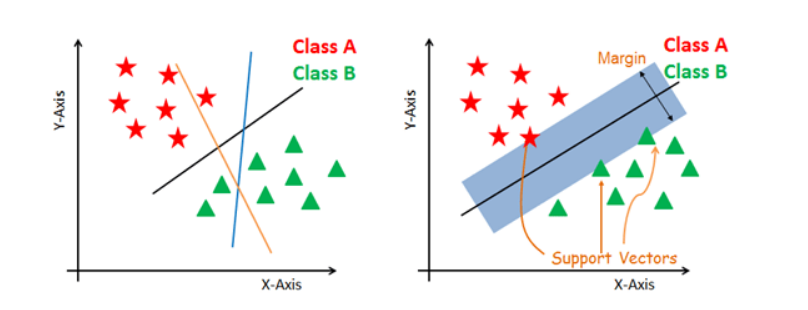
\includegraphics[]{figures/SVM.png}
\end{center}
How does an SVM work?\\

The main objective is to segregate the given dataset in the best possible way. The distance between the either nearest points is known as the margin. The objective is to select a hyperplane with the maximum possible margin between support vectors in the given dataset. SVM searches for the maximum marginal hyperplane in the following steps:

Generate hyperplanes which segregates the classes in the best way. Left-hand side figure showing three hyperplanes black, blue and orange. Here, the blue and orange have higher classification error, but the black is separating the two classes correctly.

Select the right hyperplane with the maximum segregation from the either nearest data points as shown in the right-hand side figure.

\subsection{Model Training}


\begin{itemize}
  \item Fit the training dataset on the classifier
  \item Predicted the labels on validation dataset
  \item Used accuracy\_score function to get the accuracy
\end{itemize}

\section{Results}
\begin{center}
    \begin{table}
	\begin{tabular}{ c c c c c}
		& precision & recall & f1-score & support \\
		0 & 0.87 & 0.11 & 0.20 & 1280 \\
		1 & 0.83 & 1.00 & 0.91 & 5766 \\
		accuracy & & & 0.84 & 7046 \\
		macro avg & 0.85 & 0.55 & 0.55 & 7046 \\
		weighted avg & 0.84 & 0.84 & 0.78 & 7046 \\


	\end{tabular}
	\caption{Classification Report}
    \label{Classification Report}
	\end{table}
\end{center}


It is observable from the classification report that the SVM was better at predicting the values of class 0 (Not Recommended instead of Class 1 (Recommended). The overall accuracy achieved was 84\%. The Precision is 0.84, Recall is 0.84, F1 Score is 0.78 while the support is 7046.

\section{Conclusion}
Thus, an Support Vector Machine was implemented successfully, the motive of understanding the basics of SVM and implementing it to perform a classification task was done on a dataset with satisfactory results.

\end{document}
